\documentclass[14pt]{extarticle} 
\usepackage{amsmath,mathtools,amsfonts,amsthm,amssymb,hyperref}
\usepackage{wasysym,geometry,bussproofs,latexsym,parskip,bookmark}
\usepackage{mathtools,float}
\newtheorem{defn}{Definition}
\newtheorem{thm}{Theorem}
\newtheorem{claim}{Claim}
\newtheorem{lemma}{Lemma}
\hypersetup{colorlinks,allcolors=blue,linktoc=all}
\geometry{a4paper} 
\geometry{margin=0.5in}
\title{Math for CS 2015/2019 solutions to ``In-Class Problems Week 8, Wed. (Session 19)''}
\author{https://github.com/spamegg1}
\begin{document}
\maketitle
\tableofcontents

\section{Problem 1}
A researcher analyzing data on heterosexual sexual behavior in a group of m males and f females found that within the group, the male average number of female partners was 10\% larger that the female average number of male partners.

\subsection{(a)}
Comment on the following claim. “Since we’re assuming that each encounter involves one man and one woman, the average numbers should be the same, so the males must be exaggerating.”
\begin{proof}
It may be the case that males (or females) are exaggerating (or understating), but not necessarily so.

Consider the simple bipartite graph $G = (V, E)$ of sexual liaisons between males and females. 

Then the male average number of female partners is $|E| / m$, and the female average number of male partners is $|E| / f$. If $m$ and $f$ are different, then it's normal for these averages to be different (without either sex exaggerating or understating).

So we can't say anything without knowing the actual values of $m$ and $f$.
\end{proof}

\subsection{(b)}
For what constant $c$ is $m = c \cdot f$?
\begin{proof}
The researcher found that 
$$
\frac{|E|}{m} = \frac{11}{10} \frac{|E|}{f}
$$ 
which implies that $m = \frac{10}{11}f$. So $c = 10/11$.
\end{proof}

\subsection{(c)}
The data shows that approximately 20\% of the females were virgins, while only 5\% of the males were. The researcher wonders how excluding virgins from the population would change the averages. If he knew graph theory, the researcher would realize that the nonvirgin male average number of partners will be $x(f/m)$ times the nonvirgin female average number of partners. What is $x$?
\begin{proof}
Let's write down some notation to make things clear and easy to understand.

Total male population: $m$, total male virgin population: $m_v$, total male nonvirgin population: $m_{nv}$. So $m = m_v + m_{nv}$.

Total female population: $f$, total female virgin population: $f_v$, total female nonvirgin population: $f_{nv}$. So $f = f_v + f_{nv}$.

The data says that $m_v = \frac{1}{20}\cdot m$ and $f_m = \frac{1}{5}\cdot f$. So $m_{nv} = \frac{19}{20}\cdot m$ and $f_{nv} = \frac{4}{5}\cdot f$.

Similar to before, we have that: 

the nonvirgin male average number of partners is 
$$
\frac{|E|}{m_{nv}} = \frac{|E|}{19m/20} = \frac{20}{19}\cdot\frac{|E|}{m}
$$

the nonvirgin female average number of partners is
$$
\frac{|E|}{f_{nv}} = \frac{|E|}{4f/5} = \frac{5}{4}\cdot\frac{|E|}{f}
$$

So 
$$
\displaystyle \frac{\displaystyle \frac{|E|}{m_{nv}}}{\displaystyle \frac{|E|}{f_{nv}}} = \frac{\displaystyle \frac{20}{19}\cdot\frac{|E|}{m}}{\displaystyle \frac{5}{4}\cdot\frac{|E|}{f}} = \frac{20}{19}\cdot\frac{4}{5}\cdot\frac{f}{m}
$$
\end{proof}

so $x = 16/19$.

\subsection{(d)}
For purposes of further research, it would be helpful to pair each female in the group with a unique male in the group. Explain why this is not possible.
\begin{proof}
In part (b) we found that $m < f$ so there cannot be an injective function from the set of females to the set of males.
\end{proof}

\section{Problem 2}
\subsection{(a)}
Prove that in every simple graph, there are an even number of vertices of odd degree.
\begin{proof}
1. Assume $G = (V, E)$ is a simple graph and assume $|E| = n$.

2. The sum of the degrees of all the vertices in $V$ is $2n$. (Each edge is connected to two vertices.)

3. $V$ can be separated into two disjoint subsets: $V_1 \subseteq V$ of vertices with odd degree, and $V_2 \subseteq V$ of vertices with even degree.

4. Then $\sum_{v \in V} deg(v) = \sum_{v \in V_1} deg(v) + \sum_{v \in V_2} deg(v) = 2n$.

5. Notice that $\sum_{v \in V_2} deg(v)$ is an even number (because every vertex in $V_2$ has even degree). Say it equals $2k$.

6. Therefore $\sum_{v \in V_1} deg(v) = 2n - \sum_{v \in V_2} deg(v) = 2n - 2k$ is also even.

7. So $|V_1|$ must be even: if $|V_1|$ is odd, then $\sum_{v \in V_1} deg(v)$ would also be odd (adding up an odd number of odd numbers results in an odd sum), a contradiction.
\end{proof}

\subsection{(b)}
Conclude that at a party where some people shake hands, the number of people who shake hands an odd number of times is an even number.
\begin{proof}
The people who shake hands form a simple graph under the hand-shaking relation. The people are the vertices, and there is an edge between two people if they shook hands. How many times a person shook hands corresponds to the degree of a vertex.

Therefore by part (a), the number of people who shook hands an odd number of times is odd.
\end{proof}

\subsection{(c)}
Call a sequence of people at the party a handshake sequence if each person in the sequence has shaken hands with the next person, if any, in the sequence.

Suppose George was at the party and has shaken hands with an odd number of people. Explain why, starting with George, there must be a handshake sequence ending with a different person who has shaken an odd number of hands.
\begin{proof}
???
\end{proof}

\section{Problem 3}
\begin{figure}[ht!]
\centering
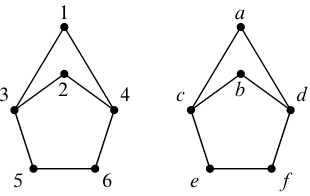
\includegraphics[scale=0.75]{isom.png}
\end{figure}

List all the isomorphisms between the two graphs given in the figure. Explain why there are no others.

\begin{proof}
Name an isomorphism $f$.

Let's look at the left graph. Nodes 3 and 4 have degree 3, and the others all have degree 2.

Let's look at the right graph. Nodes $c$ and $d$ have degree 3, and the others all have degree 2.

Since an isomorphism must preserve vertex degrees, $\{3, 4\}$ must be mapped to $\{c, d\}$. So there are 2 possibilities:

\begin{center}
$f(3) = c, f(4) = d$, or $f(3) = d, f(4) = c$.
\end{center}

The left graph has only one 4-cycle with nodes 1, 2, 3, 4 and the right graph has only one 4-cycle with nodes $a, b, c, d$. So $\{1,2,3,4\}$ must be mapped to $\{a,b,c,d\}$. 

Combining this with the above information about $\{3, 4\}$ and $\{c, d\}$, we see that there are 2 possibilities for $\{1,2\}$:

\begin{center}
$f(1) = a, f(2) = b$, or $f(1) = b, f(2) = a$.
\end{center}

Considering the only 5-cycles in the two graphs, a similar argument shows that $\{2,3,4,5,6\}$ must be mapped to $\{b,c,d,e,f\}$,  combining the above information to this, we see that $\{5,6\}$ must be mapped to $\{e,f\}$; again a similar argument shows that there are two possibilities for $\{5,6\}$:

\begin{center}
$f(5) = e, f(6) = f$, or $f(5) = e, f(6) = f$.
\end{center}

\begin{center}
$f(1) = a, f(2) = b$, or $f(1) = b, f(2) = a$.
\end{center}

Therefore there are 8 possible isomorphisms. Written in a simplified notation:
\begin{center}
$f: 123456 \to abcdef$\\
$f: 123456 \to abcdfe$\\
$f: 123456 \to abdcef$\\
$f: 123456 \to abdcfe$\\
$f: 123456 \to bacdef$\\
$f: 123456 \to bacdfe$\\
$f: 123456 \to badcef$\\
$f: 123456 \to badcfe$
\end{center}
There are no others, due to preserving edges, vertex degrees, and cycles.
\end{proof}

\section{Problem 4}
Which of the items below are simple-graph properties preserved under isomorphism?

\subsection{(a)}
The vertices can be numbered 1 through 7.
\begin{proof}
This is another way of saying that two isomorphic finite simple graphs have the same number of vertices, which is true (because an isomorphism is a bijection, which preserves cardinality). So this is preserved under isomorphism.
\end{proof}

\subsection{(b)}
There is a cycle that includes all the vertices.
\begin{proof}
Preserved under isomorphism. Because an isomorphism preserves edges between vertices.
\end{proof}

\subsection{(c)}
There are two degree 8 vertices.
\begin{proof}
Again, preserved under isomorphism. Since edges are preserved, so are vertex degrees.
\end{proof}

\subsection{(d)}
Two edges are of equal length.
\begin{proof}
Not preserved. Edges can be as long or as short as we want. An isomorphism only cares about whether or not there is an edge between two vertices, not how long that edge is.
\end{proof}

\subsection{(e)}
No matter which edge is removed, there is a path between any two vertices.
\begin{proof}
Preserved. Since an isomorphism preserves edges, it also preserves paths.
\end{proof}

\subsection{(f)}
There are two cycles that do not share any vertices.
\begin{proof}
Preserved. Paths and cycles are preserved; so are the lengths of paths/cycles. If two cycles $C_1, C_2$ in the first graph do not share any vertices but their isomorphic image cycles $D_1, D_2$ in the second graph shared a vertex, that vertex would end up having a different degree than its counterpart in the first graph, which is a contradiction.
\end{proof}

\subsection{(g)}
One vertex is a subset of another one.
\begin{proof}
Not preserved. An isomorphism only preserves the edge relation, the vertices could be any sets.
\end{proof}

\subsection{(h)}
The graph can be pictured in a way that all the edges have the same length.
\begin{proof}
Like part (d), not preserved.
\end{proof}

\subsection{(i)}
The OR of two properties that are preserved under isomorphism.
\begin{proof}
Preserved. If the OR of the two properties is true/false in the first graph, the properties will have the same truth value in the second graph, so the OR of the properties will still be true/false in the second graph.
\end{proof}

\subsection{(j)}
The negation of a property that is preserved under isomorphism.
\begin{proof}
Also preserved. If the property is true/false in the first graph, then its negation is false/true in the first graph. By the isomorphism, the property is true/false in the second graph, so its negation is false/true in the second graph. Therefore the negation of the property is preserved.
\end{proof}

\section{Problem 5 (Supplemental Problem)}
Let $G$ be a digraph. The neighbors of a vertex $v$ are the endpoints of the edges out of $v$. Since a digraph is formally the same as a binary relation on $V(G)$, the set of neighbors of $v$ is simply the image, $G(v)$, of $v$ under the relation $G$.

\subsection{(a)}
Suppose $f$ is an isomorphism from $G$ to another digraph $H$. Prove that $f(G(v)) = H(f(v))$.

Your proof should follow by simple reasoning using the definitions of isomorphism and image of a vertex under the edge relation - no pictures or handwaving.

Hint: Prove by a chain of iff’s that $h \in H(f(v))$ IFF $h \in f (G(v))$ for every $h \in V(H)$.
\begin{proof}
Let's try to understand the notation.

$v$ is a vertex in $G$. $f(v)$ is a vertex in $H$.

$G(v)$ is the set of vertices in $G$ that are connected directly to $v$ with an edge.

$f(G(v))$ is the set of vertices in $H$ obtained by applying $f$ to the vertices in $G(V)$.

$H(f(v))$ is the set of vertices in $H$ that are connected directly to $f(v)$ with an edge.

OK! Let's do it. For every vertex $h \in V(H)$, 

\begin{tabular}{ccl}
$h \in H(f(v))$ & iff & $h$ is connected to $f(v)$ in $H$ with an edge \\
& iff & $f^{-1}(h)$ is connected to $v$ in $G$ with an edge \\
& iff & $f^{-1}(h)$ is in $G(v)$ \\
& iff & $f(f^{-1}(h))$ is in $f(G(v))$\\
& iff & $h$ is in $f(G(v))$ 
\end{tabular}

We are using the fact that $f$ is an isomorphism, therefore so is $f^{-1}$.
\end{proof}

\subsection{(b)}
Conclude that if $G$ and $H$ are isomorphic graphs, then they have the same number of vertices of outdegree $k$, for all $k \in \mathbb{N}$.
\begin{proof}
1. Assume $G$ and $H$ are isomorphic graphs, via the isomorphism $f: G \to H$. Assume $k \in \mathbb{N}$.

2. Assume $v \in V(G)$ is a vertex in $G$. We want to show that $v$ has outdegree $k$ in $G$ iff $f(v)$ has outdegree $k$ in $H$.

3. Assume $v$ has outdegree $k$ in $G$. Therefore $|G(v)| = k$. Since $f$ is an isomorphism (in particular, a bijection), $|f(G(v))| = k$.

4. By part (a), $f(G(v)) = H(f(v))$. So $f(v)$ has outdegree $k$ in $H$.

5. The proof of the converse is similar (assume $f(v)$ has outdegree $k$ in $H$, prove that $v$ has outdegree $k$ in $G$).

6. So we have showed that for all $v \in V(G)$, $v$ has outdegree $k$ in $G$ iff $f(v)$ has outdegree $k$ in $H$. 

7. Since $f$ is a bijection, this implies that $G$ and $H$ have the same number of vertices with outdegree $k$. 
\end{proof}
\end{document}
